% -*-coding: utf-8 -*-
% Держать в начале каждого файла!

\documentclass[a4paper, 12pt]{extarticle}
\usepackage{metod}

\MTDSetPhysSection{Механика}
\MTDSetTitle{Определение коэффициента трения скольжения}
\MTDDesignator{М--5}
\MTDSetGrade{10}

\MTDSetAuthors{И.~Н.~Грачева, В.~И.~Гребенкин, А.~Е.~Иванов, И.~А.~Коротова,
Е.~И.~Красавина, А.~В.~Кравцов, Н.~С.~Кулеба, Б.~В.~Падалкин,
Г.~Ю.~Шевцова, Т.~С.~Цвецинская}

\MTDSetEditorsGenCase{И.~Н.~Грачевой, А.~Е.~Иванова, А.~В.~Кравцова}

\newcommand{\eps}{\epsilon}

\begin{document}

\MTDTitlePage
\MTDInfoPage

\setcounter{section}{5}

\subsection{Цель работы}
Целью работы является измерение коэффициента трения скольжения.

\subsection{Основные теоретические сведения}
Сухое трение возникает на поверхностях соприкосновения твердых тел. Сила трения имеет электромагнитную природу. Ее возникновение обусловлено межмолекулярным взаимодействием. Эта сила направлена вдоль поверхности соприкосновения.

Сила трения скольжения возникает при относительном движении соприкасающихся поверхностей и направлена противоположно относительной скорости. Этим она отличается от силы трения покоя, которая направлена противоположно приложенной силе.

Модуль силы трения скольжения пропорционален модулю нормальной силы~$N$ реакции опоры
\begin{equation}
\label{eq:m5-frictional-force}
F_\text{тр} = \mu N,
\end{equation}
где $\mu$ "--- коэффициент трения скольжения.

Выражение~\eqref{eq:m5-frictional-force} называют уравнением Амонтона. Коэффициент трения скольжения~$\mu$ не зависит от силы~$N$ и площади соприкосновения, но сильно зависит от степени шероховатости и рода вещества соприкасающихся тел.

Коэффициент~$\mu$ слабо зависит от относительной скорости поверхностей и в большинстве практических применений  этой зависимостью пренебрегают.

Сила трения скольжения является неконсервативной силой, работа этой  силы зависит от формы траектории. Сила трения скольжения направлена противоположно относительной скорости соприкасающихся тел, а значит, и противоположно перемещению одного тела относительно другого. Из  этого следует, что работа силы трения отрицательна.

\subsection{Методика проведения эксперимента и описание экспериментальной установки}
Измерение коэффициента трения скольжения производится на основе использования теоремы о кинетической энергии, в соответствии с которой изменение кинетической энергии тела равно сумме работ внешних сил, приложенных к телу.

Рассмотрим схему экспериментальной установки, приведенную на рис.~\ref{fig:m5-equipment}. На горизонтальную площадку~\emph{1} помещают брусок~\emph{2} и пружинный динамометр~\emph{4}, связанные нитью~\emph{3}. Динамометр закреплен за штырь~\emph{5}. При отодвигании бруска от динамометра пружина динамометра деформируется, и на брусок начинает действовать сила $F_\text{у}$ упругости со стороны динамометра. %куда бы F_y лучше написать, здесь странно | Посмотрел Иродова --- русские индексы прямые
После освобождения брусок будет двигаться до остановки. Во время движения бруска работу совершают сила упругости пружины~$F_\text{у}$ и сила трения скольжения~$F_\text{тр}$. Если растянутая вначале пружина динамометра окажется недеформированной, то изменение кинетической энергии бруска~$\Delta K = 0$ и конечное значение потенциальной энергии, накопленное пружиной, $\text{П}_\text{кон} = 0$, значит %ну и что с этим П делать? оно же не курсивное и вообще русское | Заменить на W или U курсивное --- от этого ничего не испортится
\begin{equation}
\label{eq:m5-law-of-conservation}
A_\text{упр} + A_\text{тр} = 0.
\end{equation}

\begin{figure}[h]
\begin{center}
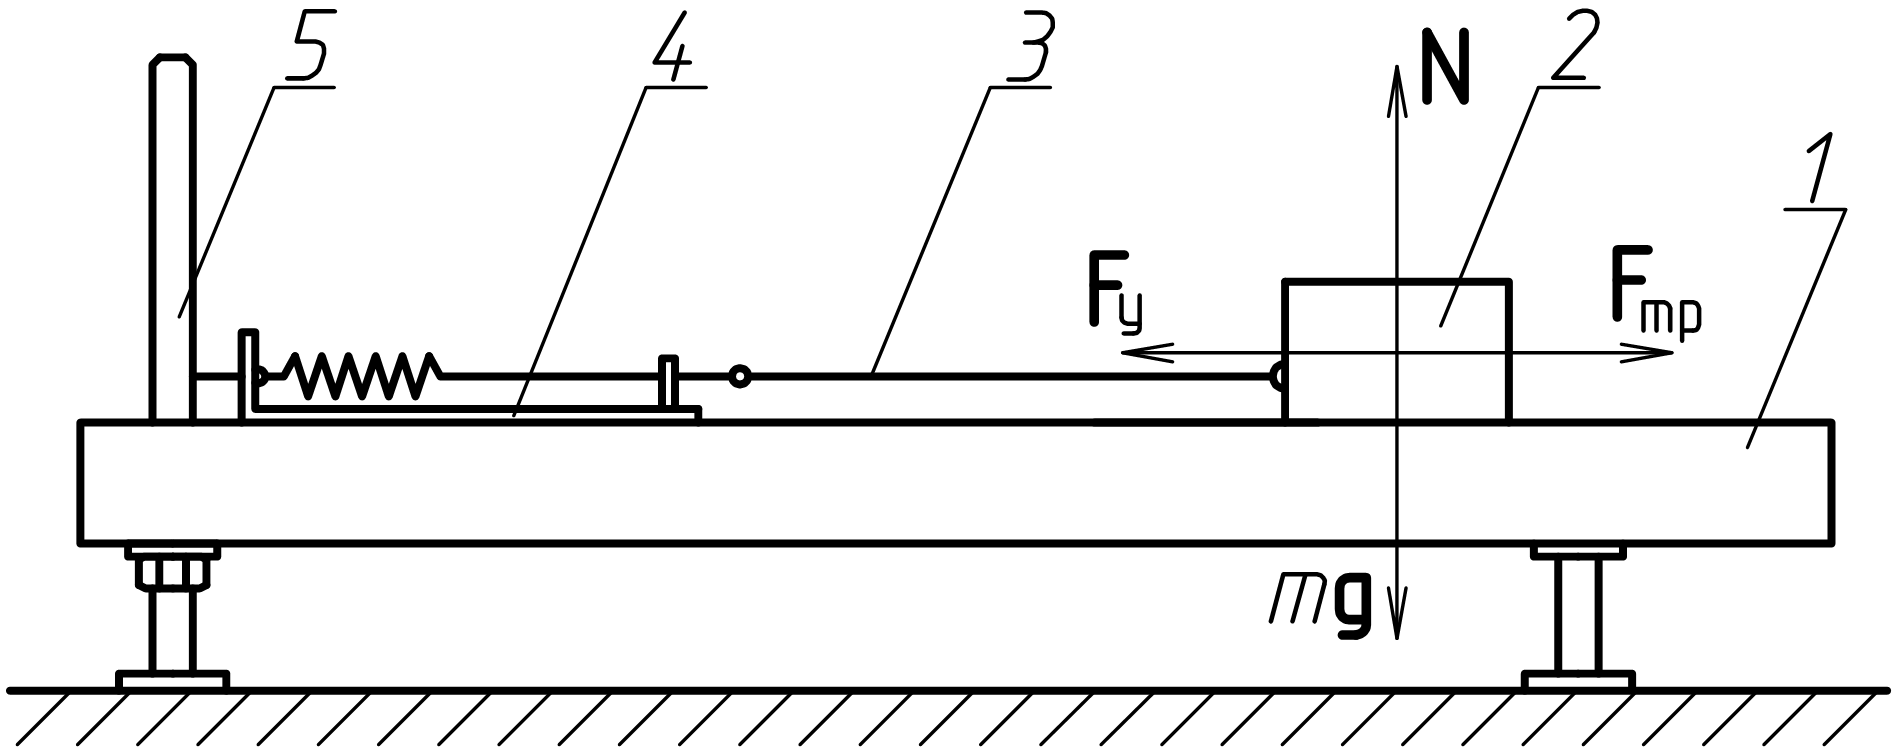
\includegraphics[scale = 0.24, keepaspectratio=true]{M5-FrictionMachine}
\end{center}
\caption{Схема экспериментальной установки \label{fig:m5-equipment}}
\end{figure} 
% ИЗМ: Убрал штриховку с кубика, вроде и без неё можно сообразить, а с ней мазня
% Не считая 

Работа силы упругости пружины связана с изменением потенциальной энергии пружины как
\begin{equation}
\label{eq:m5-work-of-elastic-force}
A_\text{упр} = \Delta \text{П} = \frac{F_\text{упр}}{2} x,
\end{equation}
где $x$ "--- деформация пружины.

Работа силы трения на пути~$s$ % Здесь не хватает двоеточия. Иначе выходит, что формула --- сказуемое ("работа" --- подлежащее), но так как формулы скорее существительные, чем глаголы, получается, что надо ставить тире... А это совсем странно. С двоеточием будет сложное предложение из двух назывных
\begin{equation}
\label{eq:m5-work-of-frictional-force}
A_\text{тр} = -\mu m g s.
\end{equation}

Из выражений (5.2)--(5.4) следует, что %а такое тех умеет делать (про выражения)? | Ссылаться? \eqref{}. Или ты не про это?
\begin{equation}
\label{eq:m5-coefficient-of-friction}
\mu = \frac{F_\text{упр} x}{2mgs}.  %упр прилип к x | Отодвинь его hspaceом или F_\text{упр } x - тоже хорошо выглядит
\end{equation}

\subsection{Порядок выполнения работы и обработки результатов измерений}
\begin{enumerate}
\item В процессе домашней подготовки подготовьте в протоколе эксперимента таблицу~\ref{tab:m5-res-exp}.

\begin{table}[h]
\caption{\label{tab:m5-res-exp}}
\begin{flushright}
\begin{tabular}{|c|c|>{\centering\arraybackslash} m{1.21cm}|>{\centering\arraybackslash} m{1.21cm}|>{\centering\arraybackslash} m{1.21cm}|>{\centering\arraybackslash} m{1.21cm}|>{\centering\arraybackslash} m{1.21cm}|>{\centering\arraybackslash} m{1.21cm}|>{\centering\arraybackslash} m{1.21cm}|}
\hline
\multirow{2}*{\textnumero \ опыта} & \multirow{2}*{\textnumero \ измерения} & \multirow{2}*{$m,~\text{\Units{кг}}$} & \multirow{2}*{$F_\text{у},~\text{\Units{Н}}$} &  \multirow{2}*{$x,~\text{\Units{м}}$} & \multirow{2}*{$s,~\text{\Units{м}}$} & \multirow{2}*{\hspace{3pt}$\MTDMean{s},~\text{\Units{м}}$} & \multirow{2}*{$\mu$} & \multirow{2}*{$\Delta \mu$} \\
      & & & & & & & & \\ \hline
\multirow{2}*{\LARGE 1} & 1 & & & & & & & \\ \cline{2-2} \cline{4-6}
      & 2 & & & & & & & \\ \hline
\multirow{2}*{\LARGE 2} & 1 & & & & & & & \\ \cline{2-2} \cline{4-6}
      & 2 & & & & & & & \\ \hline
\multirow{2}*{\LARGE 3} & 1 & & & & & & & \\ \cline{2-2} \cline{4-6}
      & 2 & & & & & & & \\ \hline
\end{tabular}
\end{flushright}
\end{table}

\item К динамометру и бруску привяжите нить длиной примерно 0,1~\Units{м}.
\item Брусок и динамометр поместите на площадку и закрепите динамометр за штырь.
\item Массу бруска запишите в таблицу~\ref{tab:m5-res-exp}. Масса бруска указана на самом бруске.
\item Оттяните рукой брусок так, чтобы показания динамометра были $F_\text{у} = 3,0~\text{\Units{Н}}$. Измерьте линейкой деформацию пружины $x$.
\item Значения $F_\text{у}$ и $x$ запишите в таблицу~\ref{tab:m5-res-exp}.
\item Заметьте положение бруска. Отпустите брусок. Измерьте линейкой путь~$s$, пройденный бруском, измеренное значение запишите в таблицу~\ref{tab:m5-res-exp}.
\item Повторите пп.~5--7.
\item Поместите на брусок дополнительный груз, масса которого указана на установке. Значение суммы масс бруска и дополнительного груза запишите в таблицу~\ref{tab:m5-res-exp}.
\item Повторите пп.~5--8.
\item Снимите дополнительный груз с бруска. Повторите пп.~5--8, но при значении силы упругости $F_\text{у} = 4,0~\text{\Units{Н}}$.
\item Для каждого опыта вычислите среднее значение~\hspace{2pt}$\MTDMean{s}$\hspace{2pt} по формуле
\begin{equation}
\label{eq:m5-mean-s}
\MTDMean{s} = \frac{s_1 + s_2}{2}
\end{equation}
\item Для каждого опыта вычислите абсолютную погрешность
\begin{equation}
\label{eq:m5-error}
\Delta \mu = \mu \sqrt{\eps_F^{2} + \eps_x^2 + \eps_m^2 + \eps_s^2}, 
%, \\ %\eps_F^2 плохо смотрится; взаимное расположение формул тоже | Сделай так: \sqrt{\eps_F^{\hspace{1.6pt}2}
%\nonumber
%\eps_F = \frac{\Delta F}{F};\ \eps_x = \frac{\Delta x}{x};\ \eps_m = \frac{\Delta m}{m};\ \eps_s = \frac{\Delta s}{s};
\end{equation}
где $\eps_F = \dfrac{\Delta F}{F}$; $\eps_x = \dfrac{\Delta x}{x}$; $\eps_m = \dfrac{\Delta m}{m}$; $\eps_s = \dfrac{\Delta s}{s}$; \\ % Я бы подставил \Delta S в \epsilon_s и это исчерпалось бы
$\Delta s = \dfrac{s_1 - s_2}{2}$; \\ %похоже, что здесь |s_1 - s_2|/2 | Да, по модулю, иначе плохо будет
$\Delta F$, $\Delta m$, $\Delta x$ "--- приборные погрешности.
\item Сравните полученные результаты, сделайте выводы, напишите заключение к работе.
\end{enumerate}

\subsection{Контрольные вопросы}
\begin{enumerate}
\item Зависит ли коэффициент трения скольжения от массы бруска и от силы упругости пружины?
\item Какие изменения нужно внести в экспериментальную установку, чтобы получить другое значение коэффициента трения скольжения?
\item Какие преобразования энергии происходят при выполнении эксперимента?
\end{enumerate}

\end{document}
